\documentclass[10pt]{article}
\usepackage{graphicx}
\usepackage[margin=1.5cm]{geometry}
\usepackage{amsmath}
\def\brcurs{{\mbox{$\resizebox{.16in}{.08in}{
\includegraphics{BoldR}}$}}}
\def\rcurs{{\mbox{$\resizebox{.16in}{.08in}{
\includegraphics{ScriptR}}$}}}

\begin{document}
\twocolumn

\title{Tuesday Warm-up: Potentials}
\author{Prof. Jordan C. Hanson}

\maketitle

\section{Memory Bank}

\small

\begin{itemize}
\item \textbf{Laplace's equation} in spherical coordinates, with azimuthal symmetry:
\begin{equation}
\frac{\partial}{\partial r}\left(r^2\frac{\partial V}{\partial r}\right) + \frac{1}{\sin\theta}\frac{\partial}{\partial \theta}\left(\sin\theta \frac{\partial V}{\partial \theta}\right) = 0
\end{equation}
\item \textbf{Multipole expansion} in spherical coordinates:
\begin{equation}
V(r,\theta) = \frac{1}{4\pi\epsilon_0}\sum_{n = 0}^{\infty} \frac{1}{r^{n+1}} \int (r')^n P_n(\cos\alpha)\rho(\mathbf{r}') d\tau'
\end{equation}
\end{itemize}

\begin{figure}
\centering
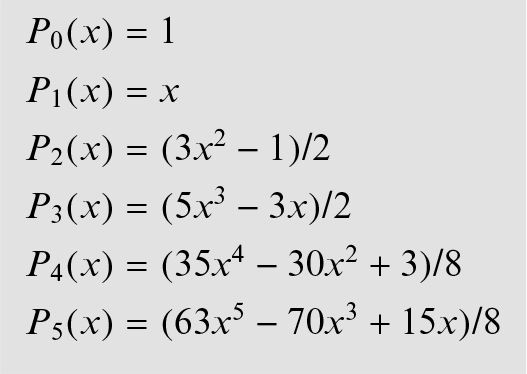
\includegraphics[width=0.2\textwidth]{figures/3_1.jpg} \hspace{0.5cm}
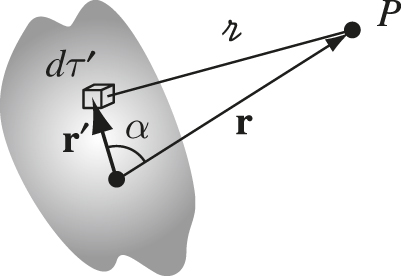
\includegraphics[width=0.15\textwidth]{figures/3_28.jpg}
\caption{\label{fig:1} (Left) The first few Legendre polynomials. (Right) The angle $\alpha$ between $\mathbf{r}$ and $\mathbf{r}'$.}
\end{figure}

\begin{figure}
\centering
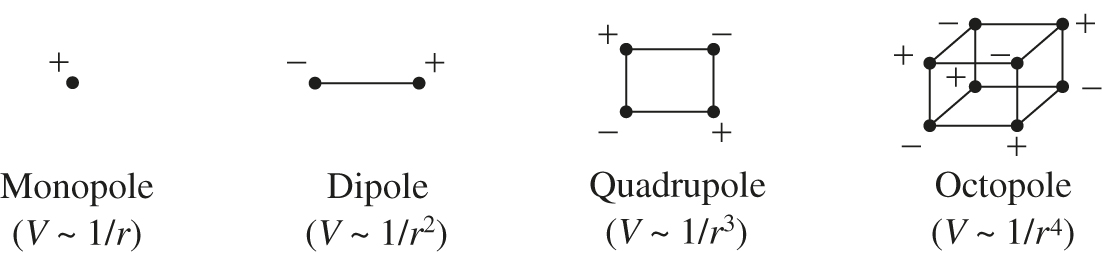
\includegraphics[width=0.49\textwidth]{figures/3_27.jpg}
\caption{\label{fig:2} Configurations of point charges.}
\end{figure}

\section{Separation of Variables}

\begin{enumerate}
\item A hollow spherical shell of radius $R$ has a potential $V_0(\theta) = V_0$ for $\theta \leq \pi/2$, and $0$ for $\theta > \pi/2$.  Find the voltage outside the shell.
\begin{itemize}
\item (a) Separate the solution for the voltage like $V(r,\theta)=R(r)\Theta(\theta)$.  Isolate the $R(r)$ and $r$ factors from the $\Theta$ and $\theta$ factors. (b) Set the ordinary differential equation for $R(r)$ equal to the constant $l(l+1)$, where $l$ is an integer.  Show that the solutions are linear combinations of $r^l$ and $r^{-(l+1)}$. \\ \vspace{2.5cm}
\item The $\Theta(\theta)$ solutions are known as \textit{Legendre polynomials}, $P_l(x)$, and $x=\cos\theta$, with the \textbf{Rodrigues} generating function
\begin{equation}
P_l(x) = \frac{1}{2^ll!}\left(\frac{d}{dx}\right)^l(x^2-1)^l
\end{equation}
Derive $P_0(x)$, $P_1(x)$, and $P_2(x)$. \\ \vspace{1.5cm}
\item Write the solution for $V(r,\theta)$ as an infinite sum, and apply the boundary condition for $r\to\infty$. \\ \vspace{2cm}
\item Apply the boundary condition at $r=R$, and use Fourier's trick to solve for the coefficients.  You will need the following orthogonality condition:
\begin{multline}
\int_{-1}^{1} P_l(x) P_l'(x) dx = \\ \int_0^\pi P_l(\cos\theta)P_l'(\cos\theta)\sin\theta d\theta = \frac{2}{2l+1}\delta_{ll'}
\end{multline}
\end{itemize}
\end{enumerate} \vspace{3cm}

\section{Multipole Expansion}

\begin{enumerate}
\item Using the multipole expansion, generate the voltage of a physical (a) monopole, and (b) dipole.  (c) What is the electric field of the dipole?
\end{enumerate}

\end{document}
